\chapter{Az \textit{Objective-C} és \textit{Swift} nyelv rövid összehasonlítása}

Szinten mindenhez lehet opcionálisan \textit{label}t hozzáadni, majd utána ennek segítségével hivatkozni rá. Ezen felül a LaTeX még automatikusan tud rakni a szám elé a/A/az/Az névelőket. Például \sectaref{objc-c-short-history} alfejezetben az Objective-C rövid története kerül bemutatásra. \sectAref{objc-c-short-history} alfejezet némiképp hiányos.

\section{Az \textit{Objective-C} nyelv rövid története}
\label{sect:objc-c-short-history}
Hivatkozhatunk könyvekre, cikkekre vagy akár weboldalakra is.\cite{UncleBob} Kép berakására ezt a snippetet ajánlom. \figAref{git-flow} képen a git-flow workflow látható.

\begin{figure}[H]
  \centering
  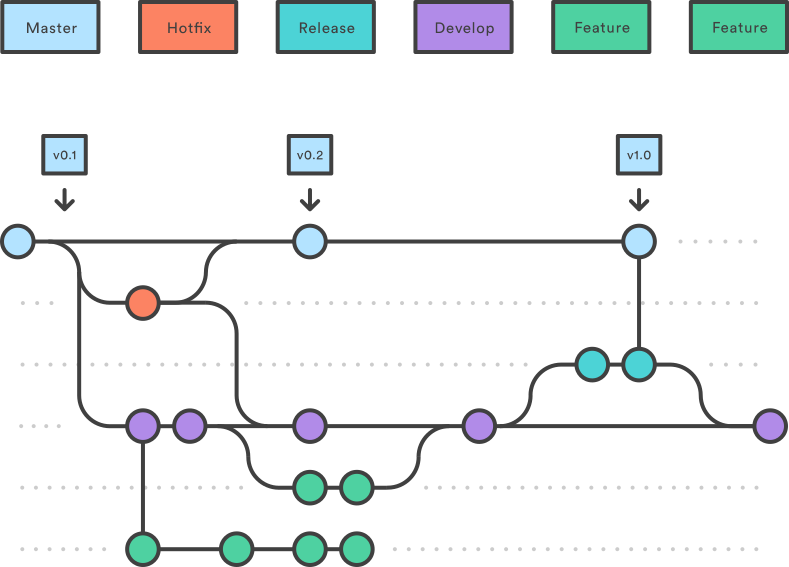
\includegraphics[width=0.7\textwidth, keepaspectratio]{figures/example_image.png}
  \caption{Git-flow workflow}
  \label{fig:git-flow}
\end{figure}

Mindenféle kódot is berakhatunk, nem mindig tökéletes eredménnyel.

\begin{otherlanguage}{english}
  \begin{code}{swift}{title={A kódrészlet "címe"}, label={lst:drop-proposal}}
func collectionView(_ collectionView: UICollectionView, dropSessionDidUpdate session: UIDropSession, withDestinationIndexPath destinationIndexPath: IndexPath?) -> UICollectionViewDropProposal {
  if collectionView.hasActiveDrag {
    return UICollectionViewDropProposal(operation: .move, intent: .insertAtDestinationIndexPath)
  } else {
    return UICollectionViewDropProposal(operation: .copy, intent: .insertAtDestinationIndexPath)
  }
}  
  \end{code}
\end{otherlanguage}

Táblázatokhoz ajánlom használni \href{https://www.tablesgenerator.com}{ezt} az oldalt:

\begin{table}[H]
  \begin{tabular}{|c|c|}
    \hline
    név        & szín       \\ \hline
    alma       & piros/zöld \\ \hline
    körte      & sárga      \\ \hline
    cseresznye & piros      \\ \hline
  \end{tabular}
\end{table}
